\chapter{Evaluation of Tree Building Methods}\label{chap:benchmark}

Whereas the variety of tree-building algorithms give evolutionists the opportunities
to choose the one that best fits the data, the disagreements between these
algorithms also confuse researchers at times. Given a set of sequences, it is not
always clear what method is most effective on a certain condition. In case
of one or a few sets of sequences, it is possible to manually curate the resultant trees.
But in the case of large-scale analysis for hundreds of gene families, such a process is formidable.
Even if massive manual curation can be achieved in the long run, which is major goal of TreeFam~\cite{li06},
guild-lines on successful tree-building are definitely beneficial to reduce manual work and
meanwhile avoid artifacts in curation.

A number of studies have been done to investigate the performance of these algorithms.
Based on the characteristics of the data sets in use, these studies can be classified into
three types: theoretical analysis on 4- or 5-leaf trees~\cite{gaut95,huelsenbeck95,yang96}, computational simulation
on large data sets~\cite{kuhner94,hall05,hollich05}, and real data from experimental manipulations~\cite{hillis92,hillis94,bull97}.
Although these studies did provide invaluable information on evaluating different algorithms, they
may still suffer a number of problems respectively: theoretical analysis can only
be applied to very small trees; computational simulation has to work with proposed evolutionary models or processes;
experiment-manipulated data are relatively small and usually developed on a special condition
that may deviate from real evolutionary processes. The most realistic evaluation is expected
to be done with large-scale data that are formed in true evolutionary history, which,
unfortunately, is unknown to us. Is there a way out?

In this chapter, we try to present a novel evaluation on various tree-building algorithms.
It differs from previous studies on two aspects: the use of large-scale curated
real data from TreeFam, and the use of model-independent indication:
duplications and losses tend to be minimized. Limited to the potential curation errors in real data and
the possibility that true evolution might favour more duplications and losses in some cases,
it is still too early to make a final conclusion about what algorithm is superior.
We only intend to show some data that will help evolutionists
to choose the most appropriate algorithms in practical use.

\section{Evaluated Algorithms and Evolutionary models}

Three classical algorithms,
distance-based method\index{tree building algorithm!distance-based},
parsimony~\cite{fitch71}\index{tree building algorithm!parsimonious} and
ML (Maximum Likelihood)~\cite{felsenstein81} method\index{tree building algorithm!maximum-likelihood},
were tested at both nucleotide level and amino acid level. Two types of merged trees were also
included. Table~\ref{tab:eval-algo} shows the 17 types of trees
used in this benchmark. More details will be explained as follows.

Distance-based method is actually the name of a group of algorithms including
Fitch-Margoliash~\cite{fitch67}\index{Fitch-Margoliash},
ME (Minimum Evolution)~\cite{rzhetsky93}\index{ME, minimum evolution},
UPGMA~\cite{sokal58}\index{UPGMA},
NJ (Neighbour-Joining)~\cite{saitou87}\index{NJ, neighbour-joining}
and several alternatives to standard NJ algorithms. In this benchmark, only standard NJ and ME
algorithms were tested in consideration of their popularity and accuracy.
NJ tree was built by NJTREE\index{NJTREE} and ME tree by FastME in GME framework~\cite{desper04}.
Distance matrix was calculated by TREE-PUZZLE~\cite{schmidt02}\index{TREE-PUZZLE}.
For nucleotide alignment, HKY~\cite{hasegawa85} model\index{HKY} was applied with
transition/transversion ratio\footnote{Transitions denote the nucleotide changes between purines
(A$\leftrightarrow$G) or between pyrimidines (C$\leftrightarrow$T),
while other types of nucleotide changes are all transversions. Biologically, transitions occur more frequently
than transversions, and therefore they are modeled differently.} estimated from data; for amino acids alignment,
WAG~\cite{whelan01}\index{WAG}
was used. In both cases, we fixed the shape factor $\alpha=1.0$ of $\Gamma$ distribution
which was approximated by 4 discrete substitution rate categories~\cite{yang94}. Alignment gaps
were regarded as missing data\footnote{Likelihood methods are capable of treating gaps as missing data
while calculating the distances. This is more robust.} in TREE-PUZZLE. As TreeFam-1.x trees were built from NJ with
p-distance\index{p-distance}\footnote{P-distance is also called mismatch distance. It actually equals to
the percent mismatches in the matched regions of two sequences.},
a distance without correction for in-site multiple substitutions\footnote{In-site multiple
substitutions denote multiple substitutions occurring at the same site.
For example, at a certain site nucleotide Adenine (A) was changed into nucleotide Guanine (G) 100 million years ago,
but 50 million years ago, the Guanine (G) was changed back to Adenine (A). Then two substitutions should be
counted even if no substitution is observed nowadays. A sophisticated evolutionary model can estimate how
often this is the case. But when sequences are too diverged, the variance of such estimation will be very large,
and therefore less accurate.}, this simplest model was also tested this time.

Parsimonious trees were reconstructed by {\bf dnapars} and {\bf protpars}, respectively.
Both programs are included in PHYLIP package~\cite{felsenstein89}\index{PHYLIP}. Tree merge
was applied if several optimal trees were given by the programs.
In our test, {\bf protpars} only presents binary trees, but {\bf dnapars} may build
multifurcated trees. As both duplication/loss inference and tree merge algorithm only work with binary trees,
some trees built by {\tt dnapars} could not be processed.

PHYML~\cite{guindon03}\index{PHYML} built ML trees. Parameters of evolutionary models are identical
to the ones used in TREE-PUZZLE. That is, HKY for nucleotide and WAG for amino acids;
substitution rates were divided into 4 discrete categories that approximated a $\Gamma$ distribution
with $\alpha=1.0$. Two or one categories were also evaluated to confirm the role
of $\Gamma$ distribution.
It seems that PHYML and TREE-PUZZLE implemented models in slightly different ways.
This can be observed when they were used to optimize branch length
given a specified tree. When we assume substitutions occur uniformly across sites (one category),
PHYML and TREE-PUZZLE can always achieve almost the same results. However,
when more than one categories are applied, their results differ more or less.
But as PHYML is unable to give a distance matrix while TREE-PUZZLE cannot
make standard ML trees, this minor inconsistency has to be tolerated.

Two trees generated by tree merge algorithm were also assessed. The first one was built by merging
a synonymous tree and a non-synonymous tree; the second by merging two ML trees and
also synonymous and non-synonymous trees. As to the objective function $f$ (Equation~\ref{equ:f-obj}),
we set $\alpha=100000$, $\beta=1000$ and $\gamma=1$. Bootstrapping values $B$ was
scaled between 0 and 100. This setting always prefers less duplications, and less losses only if
duplications are the same. Bootstrap only works when both $D^*$ and $L^*$
are identical. Due to efficiency issue, bootstrapping was not applied to
ML trees. We arbitrarily set bootstrapping support as 80 at each internal branches (branches that do not connect leaves)
given the fact that ML trees tend to be more reliable~\cite{kuhner94}.
Here, bootstrapping values are least favoured because a single tree-building algorithm
might also have high bootstrapping supports at wrong branches. Duplications are better
than losses because in evolution, duplications occur more rarely while losses more frequently, especially
following a duplication event.

\begin{table}
\begin{center}
\begin{tabular}{|l|l|}
\hline
Name & Method \\
\hline
{\tt CUR} & Curated trees from TreeFam \\
\hline
{\tt NJ-NT-HKY4} & Neighbour-Joining, HKY model, $C=4$, $\alpha=1.0$, $\kappa$ estimated \\
{\tt NJ-AA-WAG4} & Neighbour-Joining, WAG model, $C=4$, $\alpha=1.0$ \\
{\tt NJ-NT-dN} & NJ, non-synonymous distance, no correction for multi-substitutions \\
{\tt NJ-NT-dS} & NJ, synonymous distance, no correction for multi-substitutions \\
{\tt NJ-AA-MM} & NJ, p-distance (or mismatch) distance, no correction \\
{\tt NJ-AA-Kmr} & NJ, with Kimura correction \\
{\tt ME-NT-HKY4} & FastME, HKY model, $C=4$, $\alpha=1.0$, $\kappa$ estimated \\
{\tt ME-AA-WAG4} & FastME, WAG model, $C=4$, $\alpha=1.0$ \\
\hline
{\tt PAR-NT} & Parsimony (dnapars) \\
{\tt PAR-AA} & Parsimony (protpars) \\
\hline
{\tt ML-NT-HKY4} & PHYML, HKY, $C=4$, $\alpha=1.0$, $\kappa$ estimated \\
{\tt ML-NT-HKY2} & PHYML, HKY, $C=2$, $\alpha=1.0$, $\kappa$ estimated \\
{\tt ML-NT-HKY1} & PHYML, HKY, $C=1$, $\alpha=1.0$, $\kappa$ estimated \\
{\tt ML-AA-WAG4} & PHYML, WAG, $C=4$, $\alpha=1.0$ \\
\hline
{\tt MG-NT-dM} & Tree merge from {\tt NJ-NT-dS} and {\tt NJ-NT-dN} \\
{\tt MERGE} & Tree merge from {\tt ML-NT-HKY4}, {\tt ML-AA-WAG4}, {\tt NJ-NT-dN} and {\tt NJ-NT-dS}\\
\hline
\end{tabular}
\caption[Evaluated algorithms and models]{Evaluated algorithms and models. Parameter $\kappa$
	is transversion/transition ratio, $\alpha$ is the shape parameter of $\Gamma$ distribution
	which is approximated by $C$ discrete substitution rate categories.}\label{tab:eval-algo}
\end{center}
\end{table}

\section{Construction of Test Sets}
Two test sets, {\sf TestSet1} and {\sf TestSet2}, were constructed in favour of curated TreeFam families.
{\sf TestSet1} consists of 1041 trees curated in TreeFam-1. These trees were initially built
by {\tt NJ-AA-MM}. They contain genes from 12 sequenced species:
{\tt ARATH, SCHPO, YEAST, HUMAN, MOUSE, RAT, CHICK, BRARE, FUGRU, DROME, CAEBR} and {\tt CAEEL}.
The 113 trees in {\sf TestSet2} were curated based on TreeFam-2 where seven more species were added:
{\tt PANTR, CANFA, XENTR, TETNG, CIOIN, ANOGA} and {\tt APIME}. They were curated from
{\tt MERGE} trees. Besides the difference in respects of number of species and automatic methods,
trees in {\sf TestSet2} were deliberately selected such that they were neither too simple
nor too complex. In contrast, {\sf TestSet1} contains some trees that are hard to curate,
and also a lot of simple trees added at the early stage of TreeFam. This fact can be seen from
Figure~\ref{fig:leaf-dist}. Generally, {\sf TestSet2} is of higher quality.

For both test sets, original protein multialignments were directly retrieved from TreeFam.
They were converted to nucleotide alignments by matching each codon to
the corresponding amino acid. Sequences from unsequenced species were discarded.
NJTREE were used to truncate poorly aligned regions and to mask low-scoring segments.
Thompson {\it et al.}~\cite{thompson97} presented more details.

\begin{figure}
\begin{center}
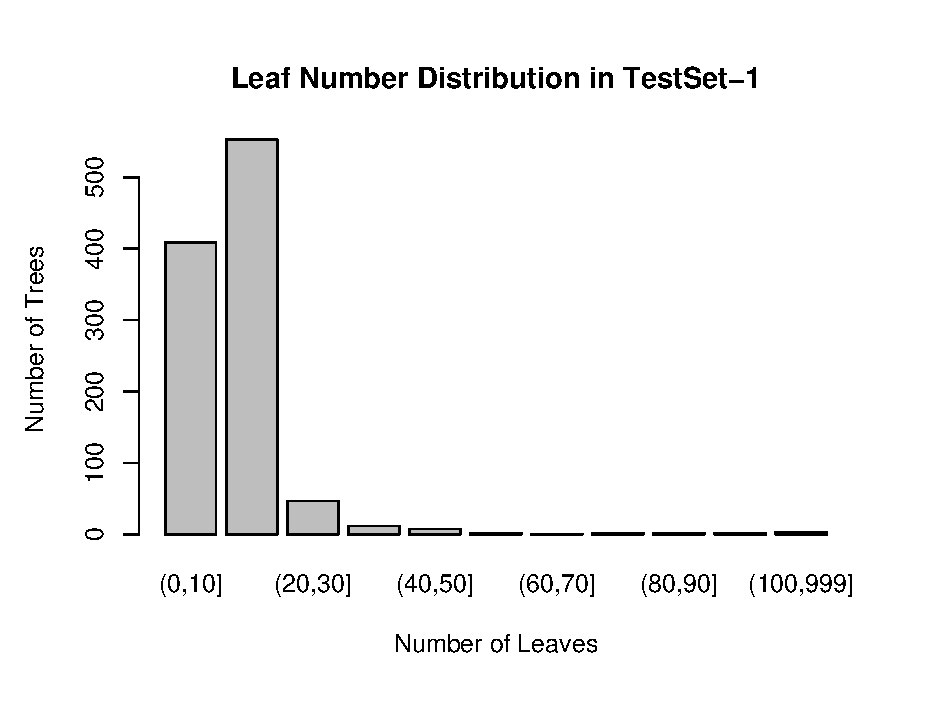
\includegraphics[width=0.49\textwidth]{leaf-ts1}
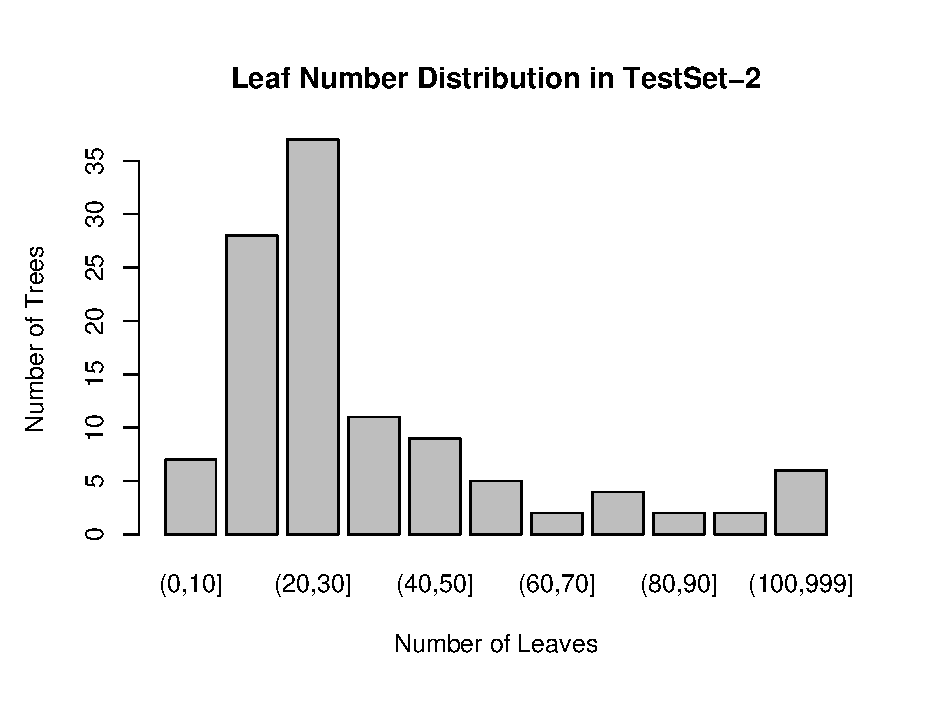
\includegraphics[width=0.49\textwidth]{leaf-ts2}
\end{center}
\caption{Distribution of number of leaves in {\sf TestSet1} and {\sf TestSet2}.}\label{fig:leaf-dist}
\end{figure}

\section{Measuring the Quality of Trees}

Two criteria were used to evaluate the quality of automatic trees. First, automatic trees were
compared with curated trees. Topological differences between them were measured by topological distance $dT$~\cite{robinson81},
which counts the number of branches that exist in one tree but not in the other~\cite{kuhner94}.
Topological distance $dT$ can be calculated given unrooted multifurcated trees. It equals to zero
if two trees are identical; it reaches its highest value $2n-6$, where $n$ is the number of
leaves in either tree, if two trees are completely different. Based on $dT$, the
distance between two methods $M_1$ and $M_2$ can be defined given $m$ multialignments:
\begin{equation}
d_M(M_1,M_2)=\frac{\sum_{i=1}^m{dT_i(M_1,M_2)}}{\sum_{i=1}^m{2n_i-6}}
\end{equation}
where $dT_i(M_1,M_2)$ is the topological distance between two trees reconstructed by the two methods based on
$i$-th multialignment, and $n_i$ is the number of sequences in the alignment.
Rescaled between 0 and 1, method distance $d_M$ is comparable between different test sets.
It, in fact, represents the percentage of branches that can only be
reconstructed by one method. In this thesis, differences between manual curation and automatic algorithms
are also measured by $d_M$.

Curated trees were processed from automatic methods. Their accuracy is inevitablely affected by
automatic methods in use. In addition, curation is a subjective process more or less, which might also make curated
trees deviate from the true history. To objectively measure the quality of automatic methods,
we also use percent duplications $p_D$ and average losses $p_L$ which are defined as:
\begin{eqnarray}
p_D(M) &=& \frac{\sum_{i=1}^m{D^*_i(M)}}{\sum_{i=1}^m{n_i-1}} \\
p_L(M) &=& \frac{\sum_{i=1}^m{L^*_i(M)}}{\sum_{i=1}^m{n_i-1}} 
\end{eqnarray}
where $D^*_i(M)$ is the number of duplications inferred from the tree reconstructed
by method $M$ from $i$-th alignment, and $L^*_i(M)$ is the number of losses. If we
accept the hypothesis that true phylogenies tend to contain fewer duplications and
losses, better methods must correspond to smaller $p_D$ and $p_L$. Although this
hypothesis might be violated in a few gene families, the overall trend should still
stand.

The two test sets only represent a small part of all Eukaryotic gene families.
To investigate the statistical reliability of our results, we designed a bootstrapping
procedure to calculate the standard deviation of each statistics, $p_D$, $p_L$ and $d_M$.
In {\sf TestSet2},
113 families were resampled with replacement for $B$ times, which forms $B$ sets of families
with each set containing 113 families.
Criterion $r_i$ was calculated from 113 resampled families for $i$-th round of resampling.
Mean value $\mu$ and SD (Standard Deviation) $\sigma$ were then estimated as:
\begin{eqnarray*}
\mu_r&=&\frac{\sum_i r_i}{B}\\
\sigma_r&=&\sqrt{\frac{\sum_i{r^2_i}-B\mu_r^2}{B-1}}
\end{eqnarray*}
A very small $\sigma_r$ means that a $r$ estimated from the original 113 families is similar to
the $r$ estimated from all animal families on the condition that these 113 families can represent all animal families.
In most cases, $\mu_r$ is almost identical to $r$ estimated from the original data, and
therefore $\mu_r$ will not be showed. Such calculation can also be applied to
{\sf TestSet1}. They are not showed as $\sigma_r$ on {\sf TestSet1} are similar to those
on {\sf TestSet2}.

\section{Accuracy of Tree Building Algorithms}

\begin{table}[!hb]
\begin{center}
\begin{tabular}{|l|cc|cc|cc|ccc|}
\hline
                 &\multicolumn{6}{|c|}{\sf TestSet2}             &\multicolumn{3}{|c|}{\sf TestSet1}\\
\hline
Type             &$d_M$ &$\sigma$&$p_D$ &$\sigma$&$p_L$ &$\sigma$&$d_M$  &$p_D$  &$p_L$  \\
\hline
{\tt CUR}        & 0.000 & 0.000 & 0.249 & 0.017 & 0.388 & 0.029 & 0.000 & 0.175 & 0.494 \\
\hline                                                                                   
{\tt NJ-NT-HKY4} & 0.225 & 0.017 & 0.313 & 0.017 & 0.786 & 0.042 & 0.133 & 0.204 & 0.630 \\
{\tt NJ-AA-WAG4} & 0.256 & 0.016 & 0.322 & 0.016 & 0.901 & 0.050 & 0.154 & 0.220 & 0.756 \\
{\tt NJ-NT-dN}   & 0.201 & 0.011 & 0.308 & 0.015 & 0.796 & 0.040 & 0.135 & 0.211 & 0.714 \\
{\tt NJ-NT-dS}   & 0.527 & 0.017 & 0.431 & 0.014 & 1.761 & 0.041 & 0.464 & 0.345 & 1.561 \\
{\tt NJ-AA-MM}   & 0.225 & 0.012 & 0.308 & 0.016 & 0.823 & 0.042 & 0.137 & 0.213 & 0.740 \\
{\tt NJ-AA-Kmr}  & 0.275 & 0.018 & 0.333 & 0.017 & 0.988 & 0.065 & 0.165 & 0.226 & 0.790 \\
{\tt ME-NT-HKY4} & 0.200 & 0.015 & 0.307 & 0.017 & 0.720 & 0.035 & 0.131 & 0.202 & 0.620 \\
{\tt ME-AA-WAG4} & 0.232 & 0.014 & 0.317 & 0.017 & 0.858 & 0.047 & 0.151 & 0.217 & 0.744 \\
\hline
{\tt PARS-NT}    & 0.203 & 0.013 & -     & -     & -     & -     & 0.151 & -     & -     \\
{\tt PARS-AA}    & 0.181 & 0.013 & 0.286 & 0.016 & 0.614 & 0.035 & 0.150 & 0.207 & 0.684 \\
\hline
{\tt ML-NT-HKY4} & 0.152 & 0.017 & 0.300 & 0.016 & 0.676 & 0.041 & 0.145 & 0.206 & 0.636 \\
{\tt ML-NT-HKY2} & 0.147 & 0.018 & 0.301 & 0.017 & 0.677 & 0.041 & 0.143 & 0.206 & 0.639 \\
{\tt ML-NT-HKY1} & 0.172 & 0.017 & 0.306 & 0.016 & 0.693 & 0.038 & 0.143 & 0.208 & 0.647 \\
{\tt ML-AA-WAG4} & 0.185 & 0.015 & 0.299 & 0.016 & 0.705 & 0.044 & 0.159 & 0.213 & 0.709 \\
\hline
{\tt NJ-NT-dM}   & 0.165 & 0.011 & 0.291 & 0.016 & 0.687 & 0.037 & 0.121 & 0.195 & 0.622 \\
{\tt MERGE}      & 0.092 & 0.015 & 0.259 & 0.016 & 0.457 & 0.033 & 0.111 & 0.178 & 0.503 \\
\hline
\end{tabular}
\caption[Performance of tree builders]{Performance of tree builders. In this table,
	$d$ is the topological distance between tree {\tt CUR} and each other tree.
	$p_D$ is percent duplication and $p_L$ the average loss. Standard deviation $\sigma$
	was calculated from 1000 times of resampling in {\sf TestSet2}. Both $p_D$ and $p_L$ are not available
	for {\tt PARS-NT} because it contains unresolved nodes.
	For $p_L$, the Pearson's correlation coefficient
	between the two sets is 0.970.}\label{tab:perform}
\end{center}
\end{table}

Table~\ref{tab:perform} shows the performance of tree-building algorithms and models.
Generally, the small SD reveals that each criterion is quite stable. Due to the
bias between {\sf TestSet2} and {\sf TestSet1}, percent duplication $p_D$ significantly
differs between the two sets. This, fortunately, does not affect the evaluation of
these algorithms. Between the two test sets, the Pearson's correlation coefficient of $p_D$ is 0.965,
and of $p_L$ is 0.970, which means that the results from the two sets highly agree with
each other.

Judged from the topological distance $d_M$ to the curated tree {\tt CUR},
tree {\tt MERGE} outperforms all the other methods on both test sets. On {\sf TestSet2},
this may be due to the fact that tree {\tt CUR} was curated from {\tt MERGE}, but
such an interpretation cannot account for the good performance on {\sf TestSet1}
where {\tt CUR} was curated from {\tt NJ-AA-MM} instead of {\tt MERGE}.
The similarity between {\tt CUR} and {\tt MERGE} on {\sf TestSet1} manifests that
human experts also favoured {\tt MERGE} even if they started from a less accurate tree.
Tree merge algorithm successfully captures the thinking of a biologist.

Judged from percent
duplication $p_D$ and average loss $p_L$, {\tt MERGE} is still the winner.
The number of duplications and losses inferred from this tree is significantly less.
The role of tree merge algorithm is also evident from {\tt NJ-NT-dM}. Merged
from {\tt NJ-NT-dN} and {\tt NJ-NT-dS}, two less accurate trees, this tree is even as accurate as those built by ML
with complex model.

So far as single-method trees are concerned, parsimony and ML methods show their power.
They are usually better than distance-based methods, except in one case where {\tt ME-NT-HKY4},
the tree built by FASTME, outperforms all the others on {\sf TestSet1}. Tree {\tt PARS-AA}
is the best on {\sf TestSet2}. But as it was merged from several parsimonious trees given by
{\bf protpars}, part of its high accuracy should attribute to the tree merge algorithm.
ML methods worked smoothly well on both sets, and on each criterion as well.
The role of applying $\Gamma$ distribution is revealed but very subtle.

As to distance-based methods, nucleotide model HKY is uniformly better than all amino acid models.
FASTME definitely outperforms standard neighbour-joining, which is in line with Desper and Gascuel~\cite{desper04}.
Notably, using complex evolutionary models at protein level does not guarantee higher accuracy at all.
This confirms the observation by Hollich {\it et al.}~\cite{hollich05}.

Figure~\ref{fig:phy-tree} shows the `phylogenies' of tree builders. `Signature' of different
tree building algorithms are evident: proteins-level methods and nucleotide-level methods
tend to be separated into two classes, while distance-based ones be grouped together.
Similar methods share similar properties. This also implies that tree merge can be more
helpful if trees with different properties are provided; otherwise common flaws
shared by a group of algorithms will never be overcome.

\begin{figure}[!hb]
\begin{center}
\includegraphics[width=\textwidth]{tree-0}\\
\includegraphics[width=\textwidth]{tree-1}
\caption[Relationships between tree builders]
{Relationships between tree builders. The top tree was built based on {\sf TestSet2}, and
the bottom on {\sf TestSet1}. Following the name of each leaf, the first number is percent duplication $p_D$
and the second average loss $p_L$. To build these two tree, topological distance $d$ between each pair of tree builders
was first calculated. Resultant distance matrix was then fed to NJTREE, which built the tree
by neighbour-joining. Bootstrapping procedure have been described above. 100 resampled
trees were finally combined together by {\bf CONSENSE} in {\bf PHYLIP} package. This
gave the supporting values on each branch.}\label{fig:phy-tree}
\end{center}
\end{figure}

\section{Discussion}
Properties of test data sets, such as divergence of sequences,
number of sequences in a tree, number of available sites in alignments,
and heterogeneity of site-specific rates, predetermine the performance
of each tree builder. This has been observed by many previous
studies~\cite{kuhner94,hall05,hollich05}. Consisting of real data from TreeFam,
our test sets represent a small number of families that date back to the last common
ancestor of Eukaryotes. Limited to the size and characteristics of data, we cannot
extensively study how each algorithm performs on various context. But as our benchmark
were carried on real data, the results may be of more practical importance.

Our work shows that tree merge algorithm is capable of
capturing the knowledge of biologists. It can greatly improve the accuracy of tree
reconstruction when the phylogeny of species is clear.
The success of tree merge also manifests that each class of single-model algorithm is able to build
part of correct branches that cannot be reconstructed by others; otherwise there must be
an algorithm that approaches the accuracy of tree {\tt MERGE}. As no single-method
algorithm can uniformly outperform all the others, it is always necessary to
combine trees with different algorithms if higher accuracy is desired.

On the other hand, tree merge only works well with Eukaryotic gene trees, where duplications
and losses can be inferred without the interference of LGT. On reconstruction of
species tree or bacterial gene trees, single-method algorithms are the only solution.
Our results suggest that each class of algorithms have their own strength. Although
parsimonious tree based on protein data and ML trees seem better in general,
distance-based method such as {\tt ME-NT-HKY4} can still outperform them at times.
Even when tree merge is not applicable, comprehensively investigating trees built
from different classes of algorithms is still always helpful.
